% KAN-ODE training loop. Compile standalone: pdflatex kan_ode_system.tex
\documentclass[tikz,border=4pt]{standalone}
\usepackage{amsmath,amssymb}
\usepackage{mathptmx}
\usepackage[scaled=0.90]{helvet}
\usetikzlibrary{arrows.meta,positioning,calc,fit,backgrounds}

\definecolor{ink}{RGB}{28,32,38}
\definecolor{primary}{RGB}{155,26,32}
\definecolor{accentsoft}{RGB}{247,228,229}
\definecolor{rule}{RGB}{209,213,219}
\definecolor{panel}{RGB}{250,250,251}
\definecolor{blueacc}{RGB}{30,90,168}
\definecolor{bluesoft}{RGB}{232,239,248}
\definecolor{muted}{RGB}{95,107,122}

\begin{document}
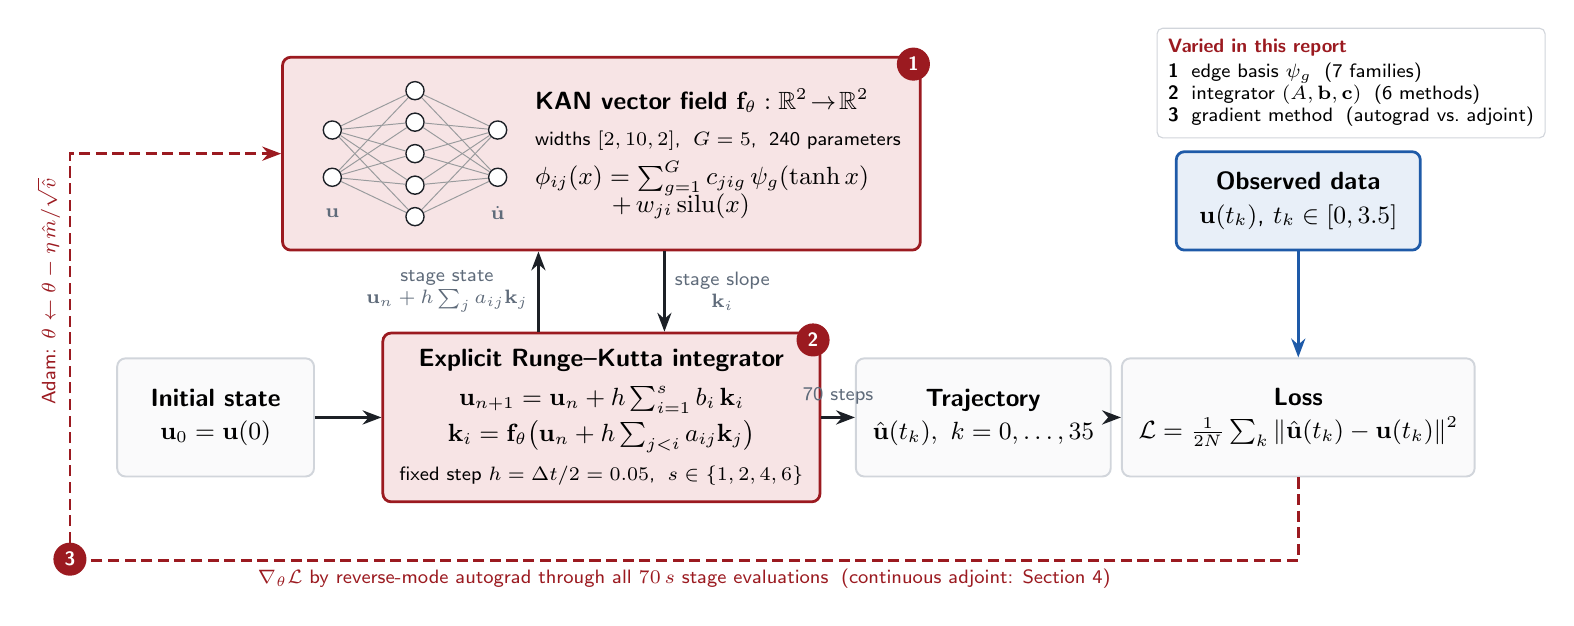
\begin{tikzpicture}[
  font=\sffamily\small, >={Stealth[length=2.4mm,width=1.8mm]},
  box/.style={draw=rule, fill=panel, rounded corners=3pt, line width=0.7pt, align=center, inner sep=6pt},
  hot/.style={draw=primary, fill=accentsoft, rounded corners=3pt, line width=1.0pt, align=center, inner sep=6pt},
  cool/.style={draw=blueacc, fill=bluesoft, rounded corners=3pt, line width=1.0pt, align=center, inner sep=6pt},
  flow/.style={->, line width=0.9pt, draw=ink},
  grad/.style={->, line width=1.0pt, draw=primary, dashed, dash pattern=on 4pt off 2pt},
  note/.style={font=\sffamily\scriptsize\color{muted}, align=center},
  badge/.style={circle, fill=primary, text=white, font=\sffamily\scriptsize\bfseries, inner sep=1.2pt, minimum size=4.2mm},
  nd/.style={circle, draw=ink, fill=white, line width=0.5pt, minimum size=2.3mm, inner sep=0pt},
]
% ------------------------------------------------------------------ nodes
\node[box, minimum width=2.5cm, minimum height=1.5cm] (u0) at (0,0)
  {\textbf{Initial state}\\[1pt] $\mathbf{u}_0=\mathbf{u}(0)$};

\node[hot, minimum width=5.0cm, minimum height=2.1cm] (rk) at (4.9,0)
  {\textbf{Explicit Runge--Kutta integrator}\\[3pt]
   $\mathbf{u}_{n+1}=\mathbf{u}_n+h\sum_{i=1}^{s} b_i\,\mathbf{k}_i$\\[2pt]
   $\mathbf{k}_i=\mathbf{f}_\theta\big(\mathbf{u}_n+h\sum_{j<i} a_{ij}\mathbf{k}_j\big)$\\[3pt]
   {\scriptsize fixed step $h=\Delta t/2=0.05$, \;$s\in\{1,2,4,6\}$}};

\node[box, minimum width=2.6cm, minimum height=1.5cm] (traj) at (9.75,0)
  {\textbf{Trajectory}\\[1pt] $\hat{\mathbf{u}}(t_k),\ k=0,\dots,35$};

\node[box, minimum width=3.1cm, minimum height=1.5cm] (loss) at (13.75,0)
  {\textbf{Loss}\\[1pt] $\mathcal{L}=\tfrac{1}{2N}\sum_k\|\hat{\mathbf{u}}(t_k)-\mathbf{u}(t_k)\|^2$};

\node[cool, minimum width=3.1cm, minimum height=1.25cm] (data) at (13.75,2.75)
  {\textbf{Observed data}\\[1pt] $\mathbf{u}(t_k)$, $t_k\in[0,3.5]$};

% KAN block with a miniature [2,10,2] network on its left
\node[hot, minimum width=8.1cm, minimum height=2.45cm] (kan) at (4.9,3.35) {};
\node[anchor=west, align=left, font=\sffamily\small] at ([xshift=3.1cm]kan.west)
  {\textbf{KAN vector field} $\mathbf{f}_\theta:\mathbb{R}^2\!\to\!\mathbb{R}^2$\\[2pt]
   {\scriptsize widths $[2,10,2]$, \;$G=5$, \;240 parameters}\\[3pt]
   $\phi_{ij}(x)=\sum_{g=1}^{G} c_{jig}\,\psi_g(\tanh x)$\\[-1pt]
   $\qquad\quad+\,w_{ji}\,\mathrm{silu}(x)$};
\begin{scope}[shift={($(kan.west)+(0.55,0)$)}]
  \foreach \k/\y in {1/-0.3,2/0.3} \node[nd] (i\k) at (0.1,\y) {};
  \foreach \k/\y in {1/-0.8,2/-0.4,3/0,4/0.4,5/0.8} \node[nd] (h\k) at (1.15,\y) {};
  \foreach \k/\y in {1/-0.3,2/0.3} \node[nd] (o\k) at (2.2,\y) {};
  \foreach \a in {1,2} \foreach \b in {1,...,5} {
    \draw[ink!45, line width=0.35pt] (i\a) -- (h\b);
    \draw[ink!45, line width=0.35pt] (h\b) -- (o\a);
  }
  \node[font=\scriptsize\color{muted}] at (0.1,-0.75) {$\mathbf{u}$};
  \node[font=\scriptsize\color{muted}] at (2.2,-0.75) {$\dot{\mathbf{u}}$};
\end{scope}

% ------------------------------------------------------------------ forward flow
\draw[flow] (u0) -- (rk);
\draw[flow] (rk) -- node[above, note, yshift=1pt] {70 steps} (traj);
\draw[flow] (traj) -- (loss);
\draw[flow, draw=blueacc] (data) -- (loss);

% stage exchange between integrator and network
\draw[flow] ([xshift=-0.8cm]rk.north) -- node[left, note] {stage state\\$\mathbf{u}_n+h\sum_j a_{ij}\mathbf{k}_j$} ([xshift=-0.8cm]kan.south);
\draw[flow] ([xshift=0.8cm]kan.south) -- node[right, note] {stage slope\\$\mathbf{k}_i$} ([xshift=0.8cm]rk.north);

% ------------------------------------------------------------------ gradient loop
\draw[grad] (loss.south) -- ++(0,-1.05) coordinate (g1) -| (-1.85,3.35) coordinate (g2) -- (kan.west);
\node[note, text=primary, anchor=north] at ($(g1)!0.5!(-1.85,-1.8)$)
  {$\nabla_\theta\mathcal{L}$ by reverse-mode autograd through all $70\,s$ stage evaluations
   \;(continuous adjoint: Section~4)};
\node[note, text=primary, rotate=90, anchor=south] at (-1.85,1.6) {Adam: $\theta\leftarrow\theta-\eta\,\hat m/\sqrt{\hat v}$};

% ------------------------------------------------------------------ what is ablated
\node[badge] at ([xshift=-3pt,yshift=-3pt]kan.north east) {1};
\node[badge] at ([xshift=-3pt,yshift=-3pt]rk.north east) {2};
\node[badge] at (-1.85,-1.8) {3};

\node[anchor=north west, align=left, font=\sffamily\scriptsize, draw=rule, fill=white,
      rounded corners=2pt, inner sep=4pt] at (11.95,4.95)
  {\textbf{\color{primary}Varied in this report}\\[1pt]
   \textbf{1}\; edge basis $\psi_g$ \;(7 families)\\
   \textbf{2}\; integrator $(A,\mathbf{b},\mathbf{c})$ \;(6 methods)\\
   \textbf{3}\; gradient method \;(autograd vs.\ adjoint)};
\end{tikzpicture}
\end{document}
